\chapter{Semi-Unsupervised Approach}

Unsupervised methods, consider a human fall as an event that deviate from normality and they are based on one-class classifiers. The main advantage of an unsupervised methods for fall detection is that it can works without knowing any examples related the the class of interest, i.e. the human fall. As aforementioned, this should be the perfect way to go in an application like this, where what we are interested in is very difficult to retrieve or we only have very few data available, but the principal weakness of an unsupervised system is that certain events deviate from normality as the human fall (e.g., the fall of an object), thus they may produce false alarms.
In this Chapter, two types of methods are described: in \secref{sec:user_aided_cin} a OCSVM used-ided method is exposed, while \secref{sec:siamese_few_shot} present an approach based on Siamese neural network for one-shot learning, both of them assessed with samples related to R0 room of the employed dataset \secref{sec:dataset}. An extension of the Siamese approach is presented in \secref{sec:siamese_few_shot} where the entire dataset presented in \secref{sec:dataset} has been used.




\section{A Combined One-Class SVM and Template Matching Approach for User-Aided Human Fall Detection}
\label{sec:user_aided_cin}

The approach proposed here, is the extension of the one presented in \secref{sec:ocsvm_approach} thus, consists of a combined One-Class Support Vector Machine (OCSVM) based method and template-matching classifier that operate in cascade. The template-matching classifier operates in a user-aided supervised manner and it is employed to reduce such errors by using a set of templates that represent these events. Templates are identified by the user that marks the occurrence of a false positive instead of a true human fall event. 
As shown in the previous section, ``unsupervised methods'' are able to overcome the need of manual tuning of ``analytical methods'' and the necessity of a large labelled dataset of ``supervised methods''. In ``unsupervised methods'', falls are discriminated from non-falls based on a model of ``normality'' constructed from a large amount of non-fall events. However, certain events differ from the ``normality'' as human falls, and they may induce the classifier to produce false alarms. As an example, \figref{fig:time_ha} and \figref{fig:spec_ha} show respectively the waveform and the spectrogram of a segment of ``normal'' human activity (footsteps and speech) \figref{fig:time_hf} and \figref{fig:spec_hf} show the waveform and the spectrogram of a segment of human fall, and \figref{fig:time_bf} and \figref{fig:spec_bf} the waveform and the spectrogram of a book fall. The figures show clearly that both falls signals differ significantly from the human activity one, thus a classifier may be induced to consider the fall of a book as the fall of a person.

\begin{figure}[htbp!]
	\centering
	\begin{subfigure}[ht]{0.5\columnwidth}
		\centering
		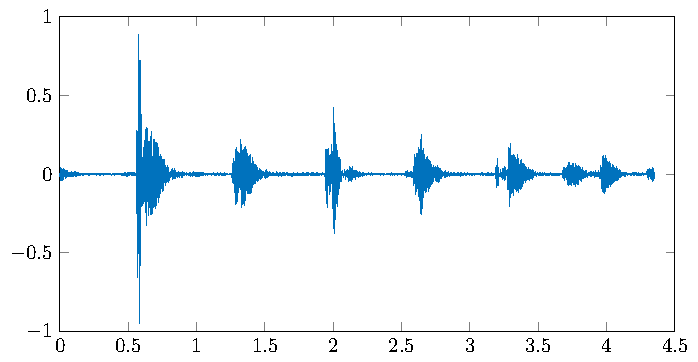
\includegraphics[width=0.9\textwidth]{img/cin/ha_time_.pdf}
		\caption{Normal human activity signal in the time domain.}\label{fig:time_ha}
	\end{subfigure}%
	\begin{subfigure}[ht]{0.5\columnwidth}
		\centering
		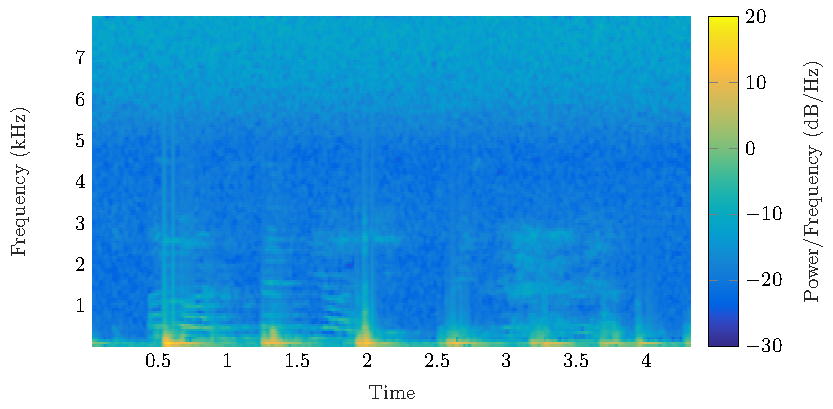
\includegraphics[width=\textwidth]{img/cin/ha_freq_.pdf}
		\caption{Normal human activity signal in the frequency domain.}\label{fig:spec_ha}
	\end{subfigure}
	
	\begin{subfigure}[ht]{0.5\columnwidth}
		\centering
		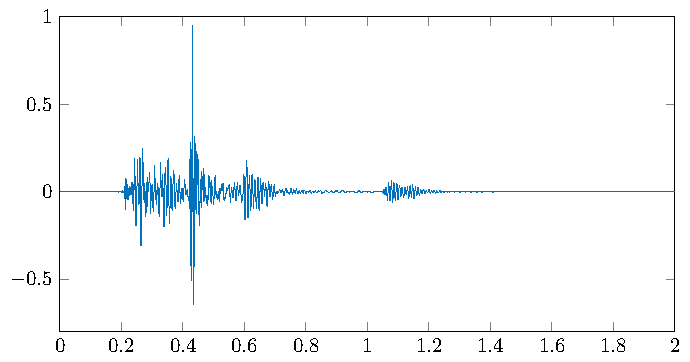
\includegraphics[width=0.9\textwidth]{img/cin/rndy_time_.pdf}
		\caption{Human fall signal in the time domain.}\label{fig:time_hf}
	\end{subfigure}%
	\begin{subfigure}[ht]{0.5\columnwidth}
		\centering
		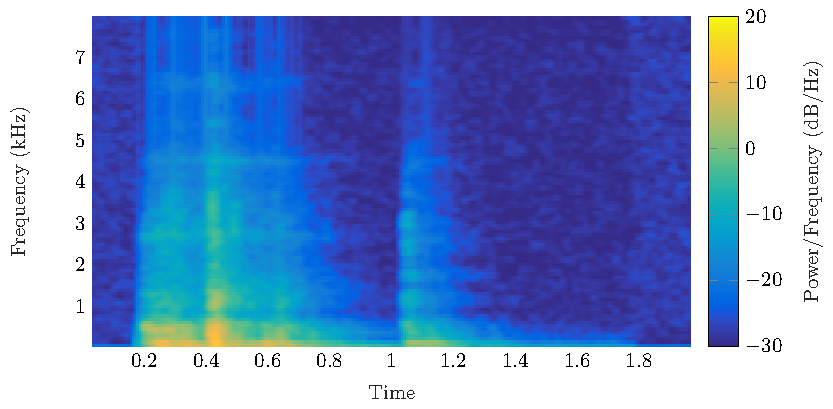
\includegraphics[width=\textwidth]{img/cin/rndy_freq_.pdf}
		\caption{Human fall signal in the frequency domain.}\label{fig:spec_hf}
	\end{subfigure}
	
	\begin{subfigure}[ht]{0.5\columnwidth}
		\centering
		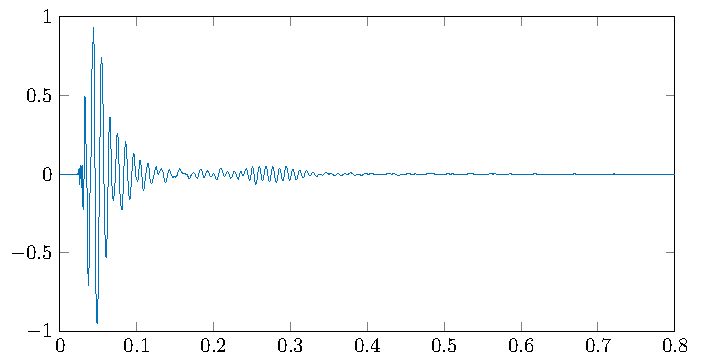
\includegraphics[width=0.9\textwidth]{img/cin/book_time_.pdf}
		\caption{Book fall signal in the time domain.}\label{fig:time_bf}
	\end{subfigure}%
	\begin{subfigure}[ht]{0.5\columnwidth}
		\centering
		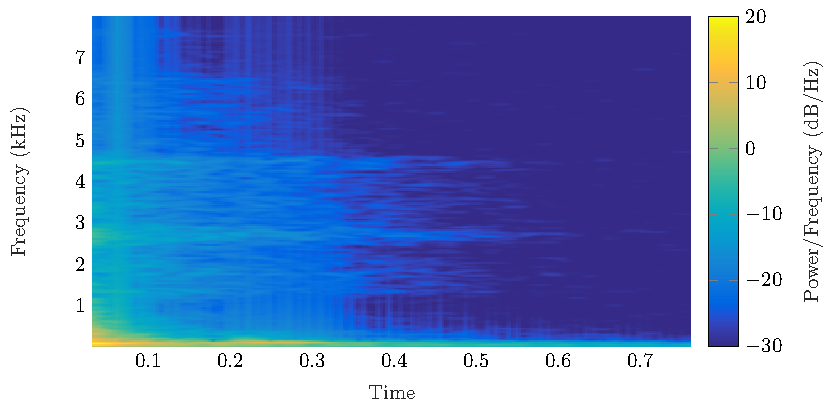
\includegraphics[width=\textwidth]{img/cin/book_freq_.pdf}
		\caption{Book fall signal in the frequency domain.}\label{fig:spec_bf}
	\end{subfigure}
	\caption{Time domain (on the left) and frequency domain (on the right) representation of a normal human activity signal (a-b), human fall signal (c-d), and book fall signal (e-f).}\label{fig:waveforms}
\end{figure}

The algorithm proposed in this paper reduces the problem by employing a multi-stage classification approach that combines a one-class classifier based on OCSVM with a template-matching stage. The OCSVM is trained unsupervisedly on a large corpus containing sounds that represent the ``normality''. On the contrary, the template-matching stage employs a set of templates represented by a small number of feature vectors marked as false alarm by the user. Thus, robustness against possible false alarms is achieved by using only few examples of false positive classes without the need of multiple sensors. An additional advantage with respect to the state of the art is that the proposed approach is able to evolve and improve after its initial training, since the template set can be augmented as non-falls events are detected.

\subsection{Proposed approach}
The proposed approach is composed of three stages \figref{fig:overall_ocsvm_user_aided}: the first (``Feature Extraction'') extracts MFCCs from the input audio signal and then GMSs to describe the entire audio segment. The second stage (``Abnormal Event Detection'') consists of a One-Class SVM classifier that discriminates between normal and abnormal sounds. Up to the authors' knowledge, OCSVM together with GMSs have never been jointly used for acoustic fall detection.  The third stage represents the innovative contribution of this paper for reducing false alarms in unsupervised approaches: it consists of a ``Template-Matching'' block that refines the output of the OCSVM and classifies the input data as fall or non-fall. The OCSVM is trained unsupervisedly on a large dataset of everyday sounds with the objective of discriminating normal from abnormal sounds. As aforementioned, the basic assumption is that the acoustic events related to human falls are ``rare'' respect to sounds normally occurring inside a home. The template-matching stage, on the other side, requires a set of ``template'' instances that represent rare events that can be confused with a fall. Referring to \figref{fig:overall_ocsvm_user_aided}, the ``Template-Matching'' stage is composed of a set of ``Templates'', a block that calculates the distance between the input GMS and the templates (``Euclidean Distance Calculation''), and a ``Decision'' block the decides whether the event is a fall or a non-fall by evaluating the magnitude of the distance.  The rationale here is that certain acoustic events are as abnormal as falls and confuse the OCSVM: the template-matching stage reduces false positives by using a set of examples related to the most confusing classes. In this work, the algorithm is ``user-aided'', i.e., templates are indicated by the user each time the OCSVM produces a false positive. This is shown in \figref{fig:overall_ocsvm_user_aided} with the person silhouette near the block that decides whether a detected fall is a false positive or not (``False Positive?''). In general, however, it is possible to create the templates set a-priori by recording several instances of possible false alarms events. Although rare, false alarm events (e.g., falls of objects) are certainly easier to reproduce in laboratory respect to human falls.

\subsubsection{Template Matching}
The template-matching classifier operates on a set of templates, i.e., supervectors, that can be defined a-priori or selected by the user when the OCSVM detects an abnormal sound that is not a human fall. Denoting with $\mathbf{x}$ the supervector of the input signal and with $\mathcal{Y} = \{\mathbf{y}_1,\ldots,\mathbf{y}_N\}$ the set of templates, the algorithm operates by calculating the Euclidean distance $D^{(i)} = \| \mathbf{x} - \mathbf{y}_i \|$ between the supervector to be classified and all the templates in the set. Indicating with $D_{min} = \underset{i}{\min}\,\,D^{(i)}$, the supervector $\mathbf{x}$ is classified as a fall if $D_{min}>\beta$ and as non-fall otherwise. The threshold $\beta$ is a hyperparameter of the algorithm that can be determined on a validation set.

\begin{figure}[ht]
	\centering
	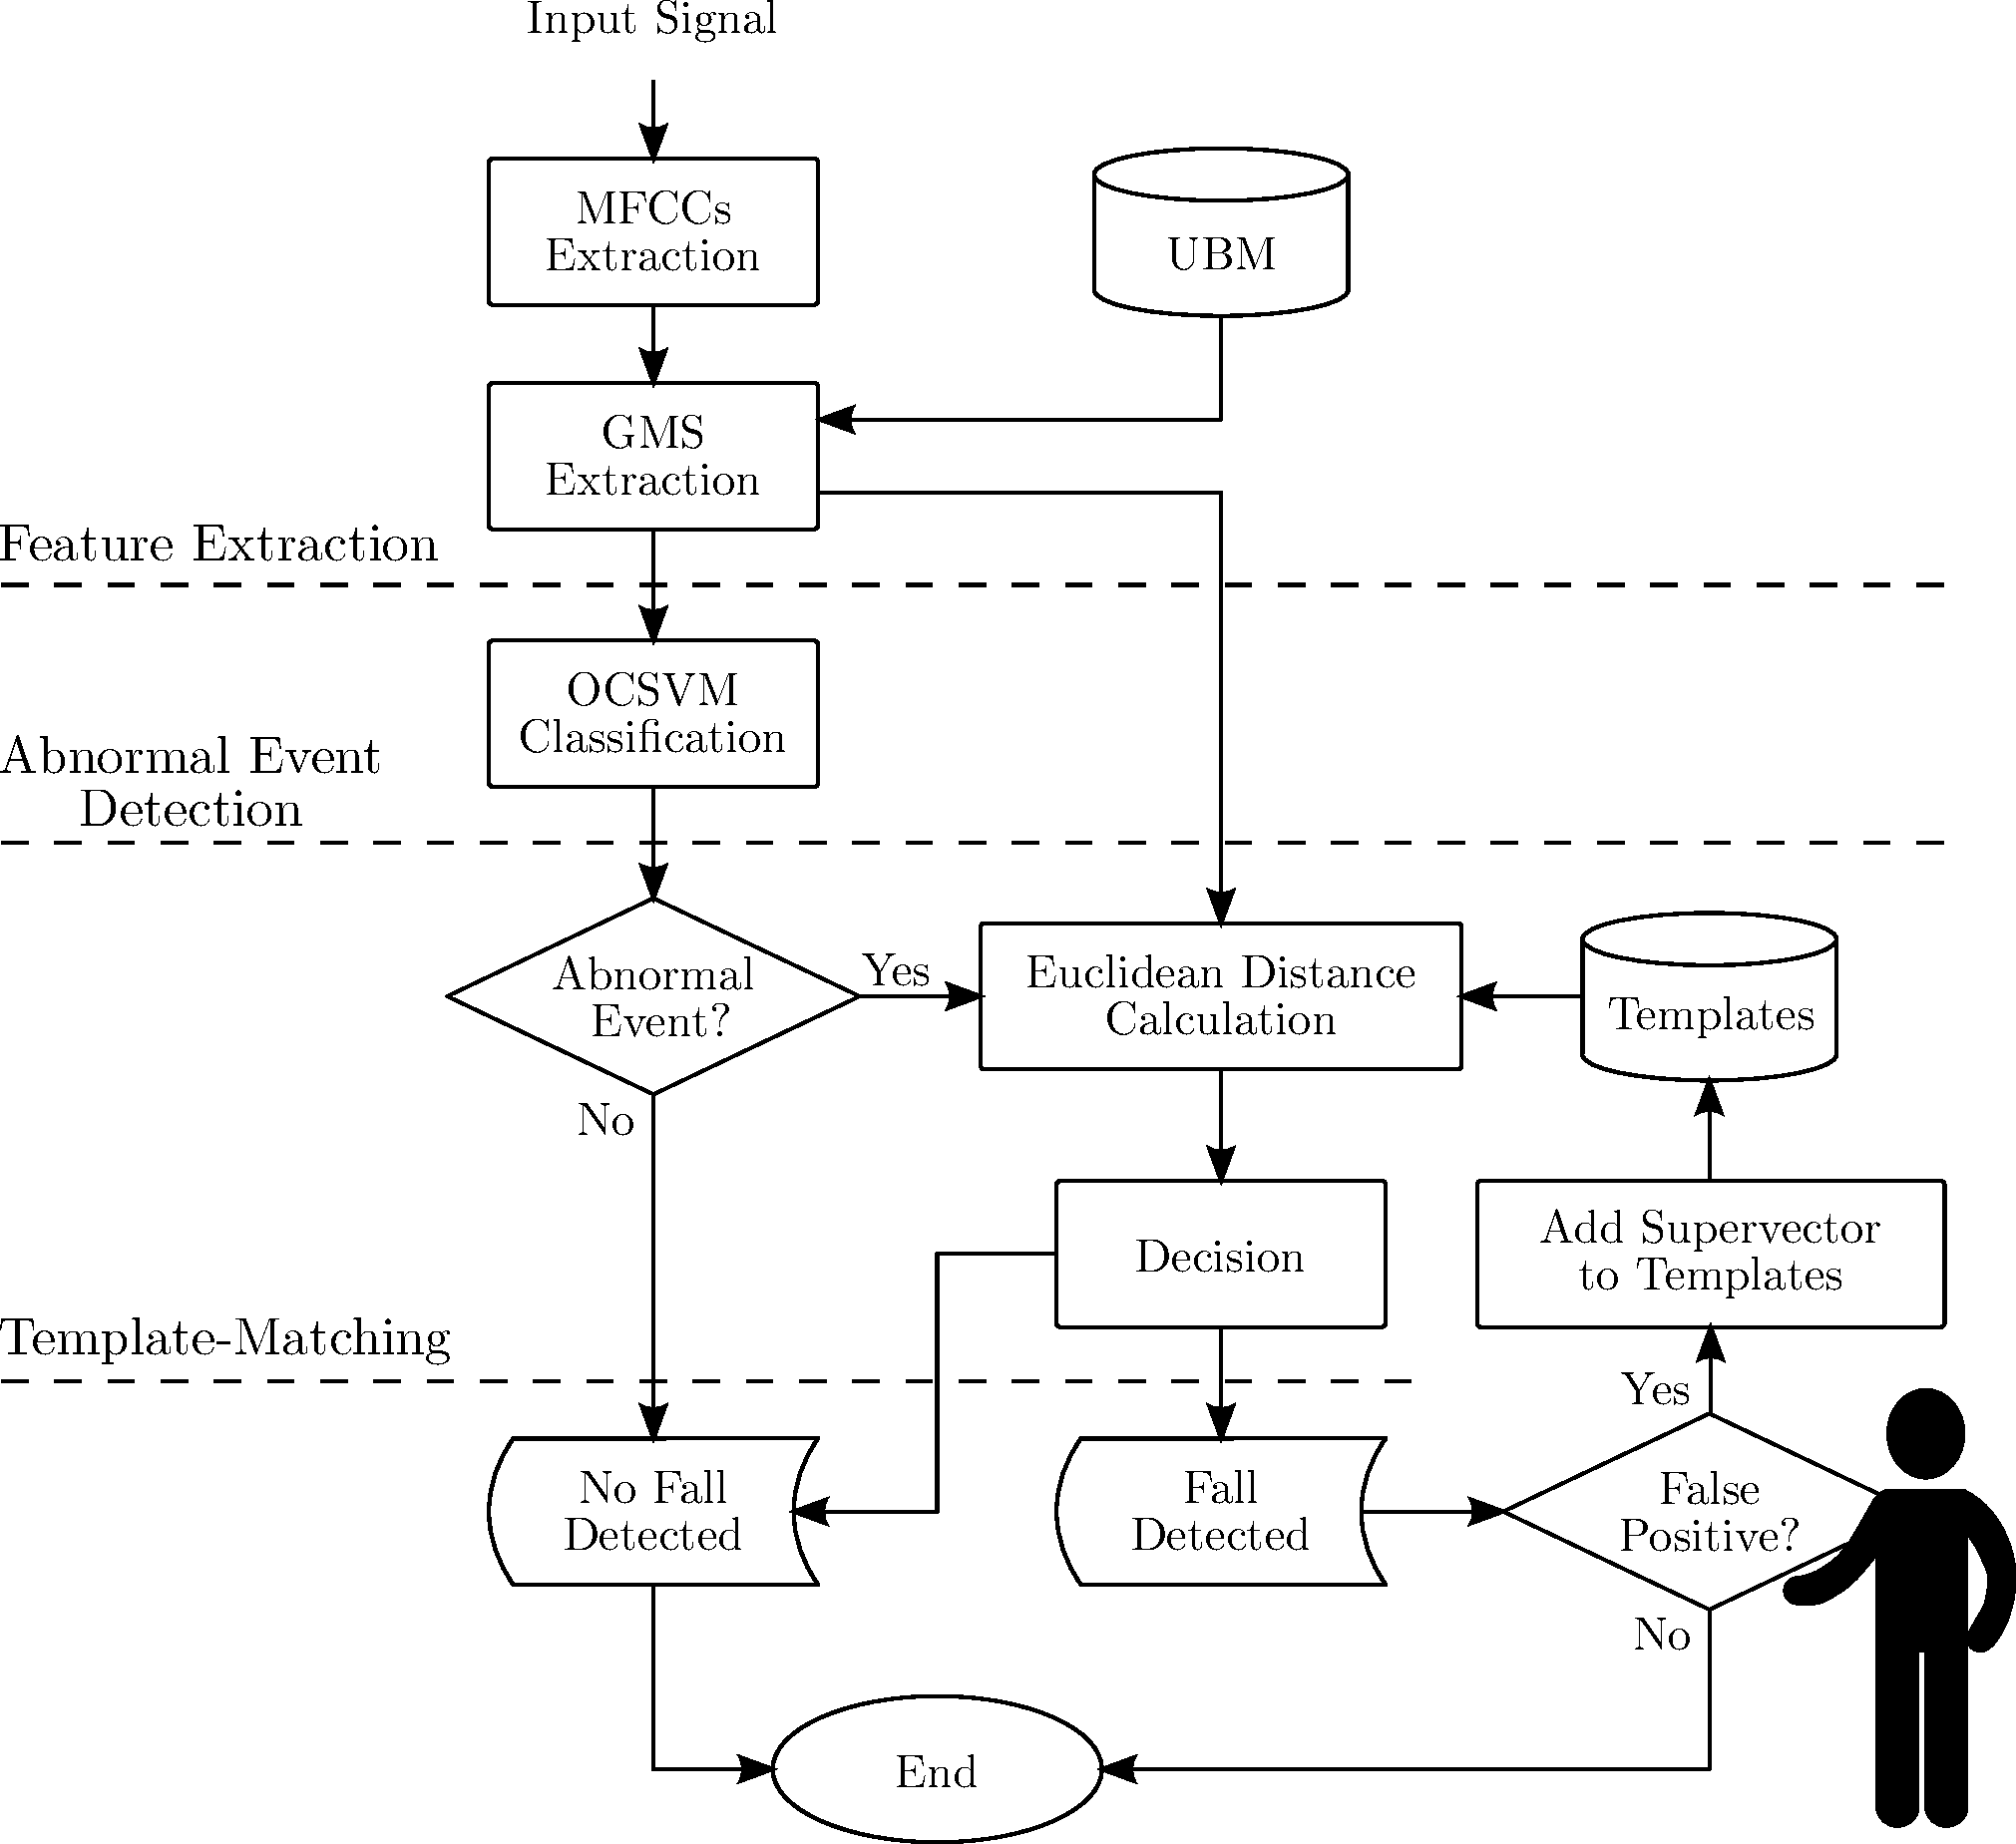
\includegraphics[width=0.95\columnwidth]{img/cin/approccioComplessivo.pdf}
	\caption{The block scheme of the proposed approach.}\label{fig:overall_ocsvm_user_aided}
\end{figure}

\subsection{Dataset}

The dataset employed in this method is the same used for the approach proposed in \secref{sec:ocsvm_approach} and reported in \tableref{tab:ocsvm_dataset}. Please refer to \secref{sec:dataset_cin_ocsvm_only} for the details.

\subsection{Experimental setup}
As in the system presented in \secref{sec:ocsvm_approach}, the dataset has been divided in one set for training the UBM and the OCSVM and three sets for evaluating the performance.
Training has been performed on the same set used for the OCSVM base algorithm presented in \secref{sec:ocsvm_approach} and shown in \tableref{tab:trainComposition}. The same three sets described in \secref{sec:experiment_ocsvm} has been used for the assessment and summarized below as a reminder:
\begin{itemize}
	\item Set 1: Human fall and background sounds (\tableref{tab:set1Composition_}).
	\item Set 2: Human fall and object fall sounds (\tableref{tab:set2Composition_}).
	\item Set 3: Human fall, object fall and background sounds (\tableref{tab:set3Composition_}).
\end{itemize}


\begin{table}[ht]
	\centering
	\caption{Data used in ``Set 1''.}
	\begin{subtable}[ht]{.6\textwidth}
		\centering		
		\caption{Composition  of ``Set 1''.}
		\label{tab:set1Composition_} % è lo stesso del capitolo 5. Lo riporto qui per comodità di lettura
		\begin{center}
			\begin{tabular}{K{3cm}K{3cm}}				
				\hline
				\textbf{Class} & \textbf{Nr.\ of occurrences} \\ 
				\hline
				$\,$ Human Falls $\,$ 	& 44    			\\
				Human Activity  		& 15		\\
				Music			  		& 29		\\
				%				 Classic Music       	& 15   		\\
				%				 Rock Music       		& 14  		\\		
				\hline
			\end{tabular}			
		\end{center}		
	\end{subtable}%
	\begin{subtable}[ht]{.6\textwidth}
		\centering		
		\caption{Templates of ``Set 1''.}\label{tab:set1Template}
		\begin{center}
			\begin{tabular}{ccc}
				
				\hline
				\multirow{2}{1cm}{\textbf{Class}}	& \multicolumn{2}{c}{\textbf{Nr.\ of templates}}	\\ 
				\cline{2-3}
				&\textbf{Clean}&\textbf{Noisy}						\\
				%& \hspace{8pt}Clean\hspace{8pt}  & \hspace{6pt}Clean\hspace{6pt}   \\ 
				\hline
				Human Activity  		& 13	&	11 		\\
				Music       	& 8   	&	16		\\
				%				 Classic Music       	& 8   	&	16		\\
				%				 Rock Music       		& 0  	&	0		\\	
				\hline
				Total					& 21  	&	27		\\
				\hline
			\end{tabular}
			
		\end{center}
	\end{subtable}
	
	
\end{table}

\begin{table}[ht]
	\centering
	\caption{Data used in ``Set 2''.}
	\begin{subtable}[ht]{.6\textwidth}
		\centering
		
		\caption{Composition  of ``Set 2''.}
		\label{tab:set2Composition_}
		\begin{center}
			
			\begin{tabular}{K{3cm}K{3cm}}
				
				\hline
				\textbf{Class} & \textbf{Nr. of occurrences} \\ 
				%& \hspace{8pt}Clean\hspace{8pt}  & \hspace{6pt}Clean\hspace{6pt}   \\ 
				\hline
				$\,$ Human Falls $\,$ 	& 44    		\\				
				Basket      			& 7           	 \\
				Fork        			& 7           	 \\
				Ball       			& 8           	 \\
				Book        			& 7          	  \\
				Bag         			& 8          	  \\
				Chair       			& 7    			\\
				
				\hline
			\end{tabular}
			
		\end{center}
		
	\end{subtable}%
	\begin{subtable}[ht]{.6\textwidth}
		\centering
		
		\caption{Templates of ``Set 2''.}
		\label{tab:set2Template}
		\begin{center}
			\begin{tabular}{ccc}
				
				\hline
				\multirow{2}{1cm}{\textbf{Class}}	& \multicolumn{2}{c}{\textbf{Nr.\ of templates}}	\\ 
				\cline{2-3}
				&\textbf{Clean}&\textbf{Noisy}						\\
				%& \hspace{8pt}Clean\hspace{8pt}  & \hspace{6pt}Clean\hspace{6pt}   \\ 
				\hline
				Basket  		& 55	&	57 		\\
				Fork       	& 39   	&	55		\\
				Ball      		& 11  	&	52		\\	
				Book  			& 26	&	57 		\\
				Bag       		& 26   	&	56		\\
				Chair       	& 86  	&	89		\\
				\hline	
				Total			& 243   &	366		\\	
				\hline
			\end{tabular}
			
		\end{center}
		
		
	\end{subtable}
	
	
\end{table}


\begin{table}[ht]
	\centering
	\caption{Data used in ``Set 3''.}
	\begin{subtable}[ht]{.6\textwidth}
		\centering
		
		\caption{Composition  of ``Set 3''.}
		\label{tab:set3Composition_}
		\begin{center}
			
			\begin{tabular}{K{3cm}K{3cm}}
				
				\hline
				\textbf{Class} & \textbf{Nr. of occurrences} \\ 
				%& \hspace{8pt}Clean\hspace{8pt}  & \hspace{6pt}Clean\hspace{6pt}   \\ 
				\hline
				$\,$ Human Falls $\,$ 	& 44    		\\				
				Basket      			& 3            	\\
				Fork        			& 4            	\\
				Ball       			& 4            	\\
				Book        			& 3            	\\
				Bag         			& 4            	\\
				Chair       			& 4    			\\
				Human Activity  		& 8   			\\
				Music			  		& 14   			\\
				%				 Classic Music       	& 7   			\\
				%				 Rock Music       		& 7   			\\
				
				\hline
			\end{tabular}
			
		\end{center}
		
	\end{subtable}%
	\begin{subtable}[ht]{.6\textwidth}
		\centering
		
		\caption{Templates of ``Set 3''.}
		\label{tab:set3Template}
		\begin{center}
			\begin{tabular}{ccc}				
				\hline
				\multirow{2}{1cm}{\textbf{Class}}	& \multicolumn{2}{c}{\textbf{Nr.\ of templates}}	\\ 
				&\textbf{Clean}&\textbf{Noisy}						\\
				%& \hspace{8pt}Clean\hspace{8pt}  & \hspace{6pt}Clean\hspace{6pt}   \\ 
				\hline
				Basket      			& 52     &  57		\\
				Fork        			& 57     &  57 		\\
				Ball       			& 19     &  55  	\\
				Book        			& 53     &  57   	\\
				Bag         			& 50     &  56    	\\
				Chair       			& 89     &	89		\\
				Human Activity  	& 11   	 &	4		\\
				Music 			      	& 4   	 &	11		\\
				%							 Classic Music       	& 4   	 &	11		\\
				%							 Rock Music       		& 0   	 &	0		\\
				\hline	
				Total						& 335   &	386		\\	
				\hline
			\end{tabular}			
		\end{center}		
	\end{subtable}
	
	
\end{table}
The validation phase has been set following the same procedure described in section \secref{sec:experiment_ocsvm}: a cross-validation composed of four fold has been used for estimating the hyperparameter and  the final performance is calculated by using the cumulative true positives, false positives, and false negatives obtained by varying the test folds.
Differently from the previous method, the validation phase consisted not only in searching for the number of components of the UBM and the parameters ($\nu$ and $\gamma$) of the OCSVM, but also the value of the threshold $\beta$ in the template-matching stage. The values assumed by these variables are summarized in \tableref{tab:parameter}.
The method employed for the template-matching decision threshold is explained in \secref{ssec:templateThreshold}.

%\subsection{Comparative method}

\begin{table}[ht]
	\centering
	\caption{Hyperparameters of the algorithm and search space explored in the validation phase. The search space of the template-matching threshold $\beta$ is not reported, since is determined with the procedure described in \secref{ssec:templateThreshold}. }
	\label{tab:parameter}
	\begin{tabular}{c |c | c}
		\hline
		\textbf{Stage} & \textbf{Hyperparameter} & \textbf{Range} \\
		\hline
		UBM & $J$ & $1, 2, 4, \ldots , 64$\\
		\hline
		\multirow{2}{*}{OCSVM} & $\nu$ & $0.1, 02, \ldots, 1.0$ \\
		&$\gamma$ & $2^{-15}, 2^{-13}, \ldots,2^{3} $ \\
		\hline
		Template-matching & $\beta$  & See \secref{ssec:templateThreshold}\\
		\hline
	\end{tabular}
\end{table}

All the aforementioned datasets require a set of templates for the template-matching stage of the algorithm. In the case of object falls, the set of templates has been created by classifying a set of 372 object falls with the OCSVM and selecting the occurrences misclassified as human falls. In the case of background sounds, the set of templates has been created by calculating the Euclidean distance between each occurrence of the development-set and each occurrence of a set of 470 background signals and then selecting the segment whose distance is minimum. Details on the templates sets are shown in \tableref{tab:set1Template}, \tableref{tab:set2Template}, and \tableref{tab:set3Template} respectively for ``Set 1'', ``Set 2'', and ``Set 3''.


The proposed approach has been compared with the method from which it derives (\secref{sec:ocsvm_approach}) and the algorithm presented in \cite{Popescu2009} based on OCSVM (please revert to \paragref{par:popescu_mod} for the details) 

The performance has been evaluated in terms of F$_1$-Measure \eqref{eq:f1} 

\subsection{Choice of the template-matching decision threshold}\label{ssec:templateThreshold}
A key point of the proposed approach is the decision threshold $\beta$ in the template-matching stage. Choosing a too low value would result in a low number of false negatives and a high number of false positives. On the contrary, a too high value would result in a high number of false negatives and a low number of false positives. The choice of $\beta$ has been performed by calculating the minimum Euclidean distance between each fall and non-fall event in the validation set and the set of templates. \figref{fig:distr_clean} and \figref{fig:distr_noisy} show respectively the probability distributions for the three sets in clean and noisy conditions. The decision threshold $\beta$ has been chosen at the intersection point between the distribution of fall and non-fall distances. This choice represents a compromise that balances false positives and false negatives.

Observing clean condition distributions, in ``Set 1'' the two density are considerably overlapped, while in ``Set 2'' the overlap is modest. It is expected that the possible improvement of the template-matching stage will be more consistent for ``Set 2'' respect to ``Set 1''. ``Set 3'' contains human activity and music occurrences as ``Set 1'' and object falls as ``Set 2'': indeed, the probability distributions (\figref{fig:distr_clean_set3}) are more distinct respect to the ones of ``Set 1'', but not so much as the ones of ``Set 2''.

Noisy condition distributions, shown in \figref{fig:distr_noisy}, are in general less distinct compared to clean condition ones. The effect of noisy is to flatten the distances of the fall and non-fall classes, thus resulting in a less discriminative capabilities of the classifier. Thus, it is expected that the performance improvement in noisy conditions will be more modest respect to the one obtained in clean condition.

\begin{figure}[ht]
	\centering
	\begin{subfigure}{0.9\columnwidth}
		\centering
		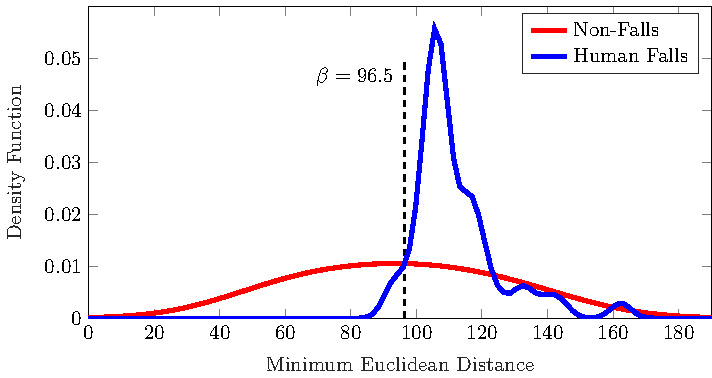
\includegraphics[width=0.98\columnwidth]{img/cin/distribuzione_Caso1_Clean.pdf}
		\subcaption{Probability distributions related to ``Set~1''.}\label{fig:distr_clean_set1}
	\end{subfigure}\hspace{1pt}
	\begin{subfigure}{0.9\columnwidth}
		\centering
		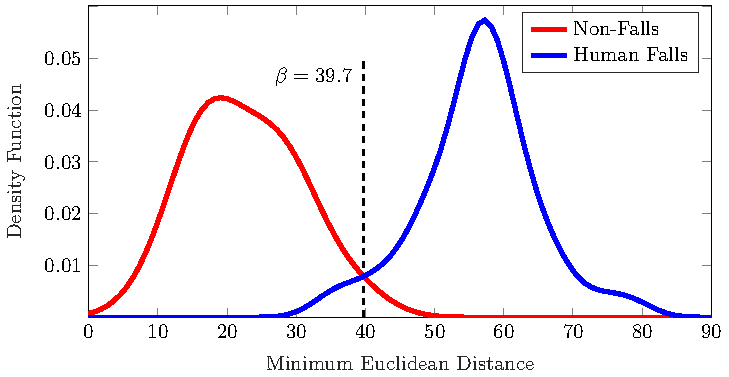
\includegraphics[width=\columnwidth]{img/cin/distribuzione_Caso2_Clean.pdf}
		\subcaption{Probability distributions related to ``Set~2''.}\label{fig:distr_clean_set2}
	\end{subfigure}\hspace{1pt}
	\begin{subfigure}{0.9\columnwidth}
		\centering
		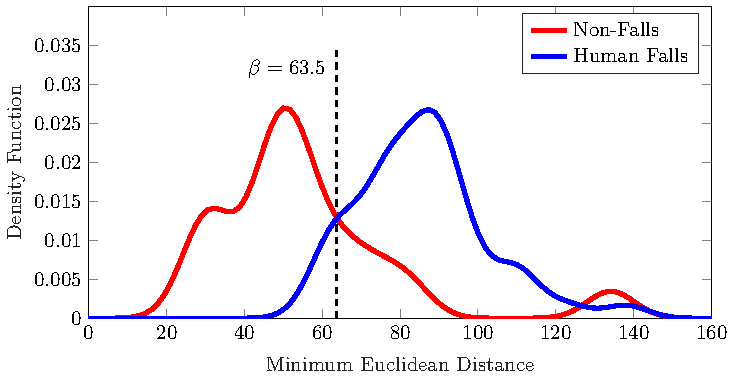
\includegraphics[width=\columnwidth]{img/cin/distribuzione_Caso3_Clean.pdf}
		\subcaption{Probability distributions related to ``Set~3''.}\label{fig:distr_clean_set3}
	\end{subfigure}
	\caption{Probability distributions of the minimum Euclidean distances among the template sets, and human falls and non-falls in \textit{clean} acoustic condition.}\label{fig:distr_clean}
\end{figure}

\begin{figure}[ht]
	\centering
	\begin{subfigure}{0.9\columnwidth}
		\centering
		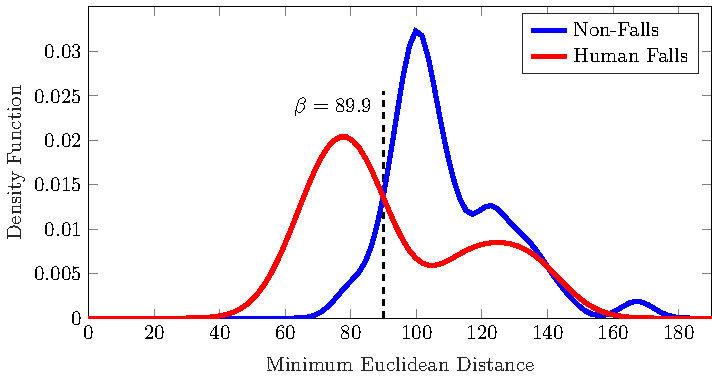
\includegraphics[width=0.98\columnwidth]{img/cin/distribuzione_Caso1_Noisy.pdf}
		\subcaption{Probability distributions related to ``Set~1''.}
	\end{subfigure}\hspace{1pt}
	\begin{subfigure}{0.9\columnwidth}
		\centering
		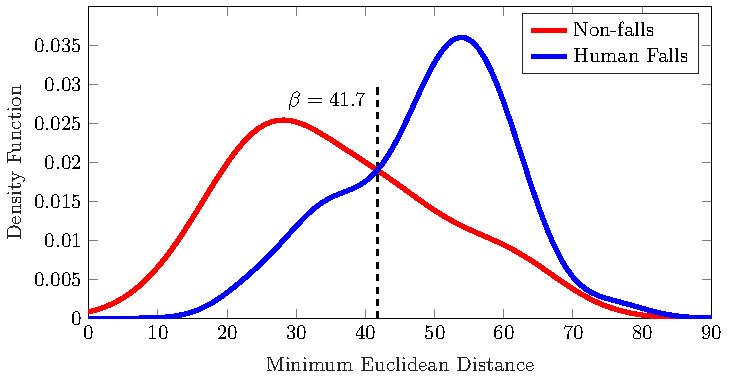
\includegraphics[width=\columnwidth]{img/cin/distribuzione_Caso2_Noisy.pdf}
		\subcaption{Probability distributions related to ``Set~2''.}
	\end{subfigure}\hspace{1pt}
	\begin{subfigure}{0.9\columnwidth}
		\centering
		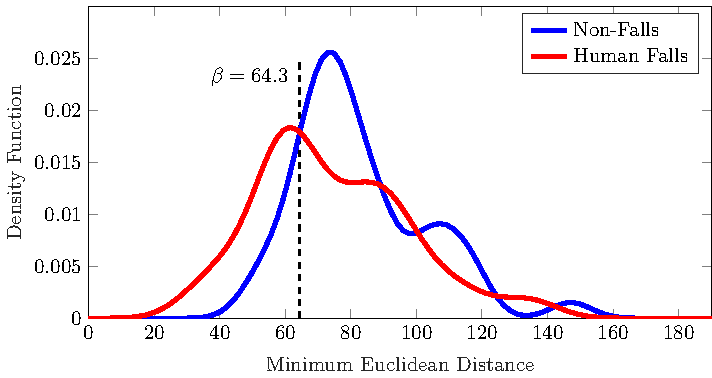
\includegraphics[width=\columnwidth]{img/cin/distribuzione_Caso3_Noisy.pdf}
		\subcaption{Probability distributions related to ``Set~3''.}
	\end{subfigure}%
	\caption{Probability distributions of the minimum Euclidean distances among the template sets, and human falls and non-falls in \textit{noisy} acoustic condition.}\label{fig:distr_noisy}
\end{figure}

\subsection{Results}
\figref{fig:res_clean_} shows the results in clean conditions obtained with and without the template-matching stage, respectively denoted as ``OCSVM+Template-Matching'' and ``OCSVM''. The results obtained with the method proposed in \cite{Popescu2009} are denoted with ``Popescu (2009)''. Observing the figure, it is evident that in all the three cases the template-matching approach is able to improve the performance with respect to ``Popescu (2009)'' \cite{Popescu2009} and the OCSVM only approach. In particular, in ``Set 1'', that comprises human falls, human activities and music, the performance improves by 2.03\% with respect to OCSVM and by 19.64\% with respect to ``Popescu (2009)''. This case can be considered as the least challenging of the three, since non-falls events are considerably different from falls ones. Conversely, ``Set 2'' comprises both human falls and object falls, thus it includes abnormal events whose pattern is similar to the one of human falls. The introduction of the template-matching stage considerably reduces the number of false positives, leading to an overall performance improvement of 20.76\%. ``Set 3'' comprises human falls, human activities, music and object falls and represents the most realistic test condition of the three. Introducing the template-matching stage, the performance improves by 7.64\%, leading to an F$_1$-Measure equal to 89.89\%. 

\begin{figure}[ht]
	\centering
	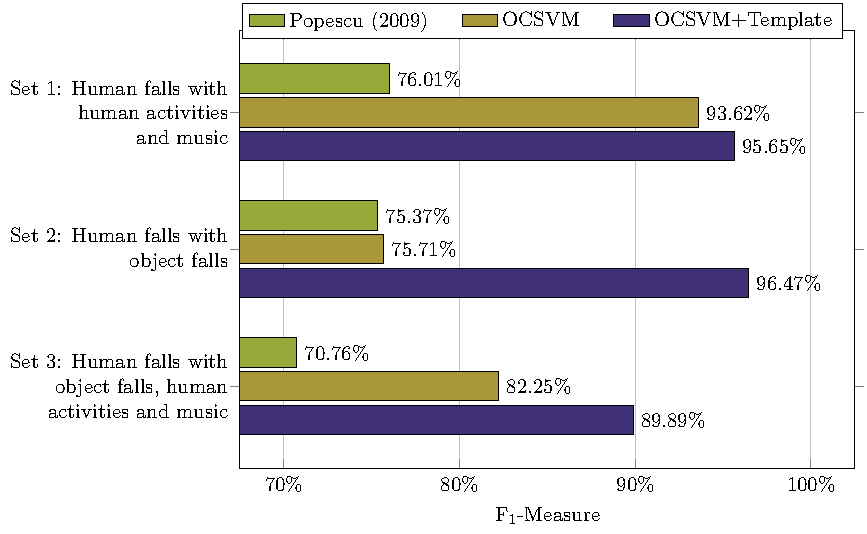
\includegraphics[width=\columnwidth]{img/cin/res_clean.pdf}
	\caption{Results in \textit{clean} conditions for the three test cases. ``Set 1'' comprises human falls, human activities and music. ``Set 2'' comprises human falls and object falls. ``Set 3'' comprises human falls, object falls, human activities, and music.} \label{fig:res_clean_}
\end{figure}

\figref{fig:res_noisy_} shows the results obtained for the three cases in noisy conditions. As expected, the performance decreases in all the three evaluated methods. In ``Set 1'', the performance decrease is modest (2.32\% for the OCSVM, 2.63\% for the proposed approach, and 1.44\% for ``Popescu (2009)''), demonstrating that the OCSVM is able to effectively reject non-fall events corrupted by music interference. The use of the template-matching stage increases the performance by 1.72\%, thus providing a significant improvement also in noisy conditions. In ``Set 2'', Template-matching provides a performance improvement of 8.02\% with respect to the OCSVM, leading to an F$_1$-Measure higher than 70\%. The improvement is lower with respect to the clean ``Set 2'', since the variability of the music interference makes the Euclidean distances of fall and non-fall classes more similar and is not sufficient to overcome the ``Popescu (2009)'' \cite{Popescu2009}. In ``Set 3'', the proposed approach improves the performance by 4.77\% with respect to OCSVM and by 8.68\% with respect to ``Popescu (2009)''.

In summary, the results demonstrated that the introduction of a template-matching stage significantly improves the performance both of the OCSVM only approach and of the method by Popescu and Mahnot \cite{Popescu2009}: averaging the results over ``Set 1'', ``Set 2'', and ``Set 3'', the absolute improvement with respect to the former is 10.14\% in clean conditions and 4.84\% in noisy conditions. With respect to the latter \cite{Popescu2009} the improvement is 19.96\% in clean conditions and 8.08\% in noisy conditions. As shown in \figref{fig:res_clean_} and \figref{fig:res_noisy_}, both in clean and noisy conditions the F$_1$-Measure of the method by Popescu and Mahnot \cite{Popescu2009} is close to 75\% in ``Set 1'' and ``Set 2'', and close to 71\% in ``Set 3''. The different behaviour compared to the OCSVM only approach can be attributed firstly to the different feature representation of the audio signal (MFCCs instead of supervectors). Secondly, to the strategy adopted for classification: in \cite{Popescu2009}, signals are divided in windows and a fall is detected if at least two consecutive windows are classified as fall. Differently, in the proposed algorithm, the overall signal is represented by a single supervector and classified as fall or non fall.

Comparing the results in clean (\figref{fig:res_clean_}) and noisy (\figref{fig:res_noisy_}) conditions, it is evident that techniques for reducing the impact of additive noise are needed. Additionally, the proposed solution requires the intervention of the user for selecting the templates after the first classification stage performed by the OCSVM. This aspect will be addressed in next sections in order to make the algorithm completely independent of the user, using a low number of examples related to human fall.

\begin{figure}[ht]
	\centering
	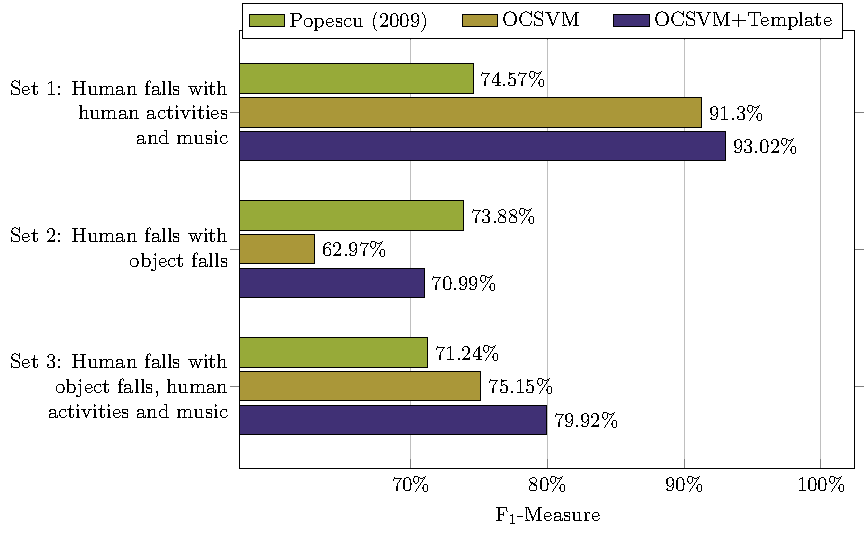
\includegraphics[width=\columnwidth]{img/cin/res_noisy.pdf}
	\caption{Results in noisy conditions for the three test cases. ``Set 1'' comprises human falls, human activities and music. ``Set 2'' comprises human falls and object falls. ``Set 3'' comprises human falls, object falls, human activities, and music.} \label{fig:res_noisy_}
\end{figure}


\section{Few-shot Siamese Neural Networks employing Audio features
for Human-Fall Detection}
\label{sec:siamese_few_shot}
As already mentioned, the main challenge for falls detector systems is the lack of human falls examples in the dataset, that are rare and hardly recoverable. Hence the need to develop systems that are able to work with no or few such data. In fact, Khan et al. \cite{khan2017review} analyze Fall Detection techniques and divides them based on data availability prospective in two groups. The group is composed of algorithms that can draw form dataset with sufficient number of human falls that can be used in training. Mostly based on supervised machine learning, thresholding and one-class techniques, this methods attempt to detect a fall directly given their training data. As we show here, although these supervised techniques can achieve a high reliability, they needs a large labelled dataset including many human fall, that is not easy to retrieve for this specific application. Moreover, applying this techniques when there are no training data for human falls leads to an unacceptable miss rate. As a comparative model for this category, has been evaluated an algorithm based on SVM.% described below %that shows good results in \cite{Principi2016a}
. The second group include algorithms that can draw form dataset with insufficient or no training data for falls mostly based on over/under-sampling, semi-supervised learning, novelty detection and one-class classification. Those techniques differ from the previous ones because uses the available data as a description of normal activities. Once it is trained on these data, can be able to classify a test sample as a human fall or non-human fall. The major drawback here is that they need a good description of what ``normal activities'' are. In fact to give a good representation of this concept, a big data set comprising all the normal activities is needed \cite{pimentel2014review}. In real scenario, this is very difficult to obtain and this may induce the classifier to produce a high number of false alarms. As a comparative models for this category, 2 approaches have been evaluated: a OCSVM that is a totally unsupervised method and a extremely unbalanced SVM that use only one human fall for the training phase%, both described below.
.

The proposed algorithm belongs to the second category, and as a first step, we demonstrate that the SNN can achieve better results than both unsupervised and supervised methods when they are tested under similar conditions.


%Learning a Similarity Metric Discriminatively, with Application to Face Verification
% quello di lecunn e ella contrastive loss
%One-Shot Learning of Object Categories 
% del 2006
%One-shot Learning with Memory-Augmented Neural Networks
%altro lavoro su one shot learning
%Matching Networks for One Shot Learning
%altri lavori sepre su immagini per il one shot (non siamesi)
One-shot or few-shot methods have been recently revived in other fields of application.
The Siamese approach was introduced by Bromley et al. \cite{bromley1994signature} for signature verification and later also used in \cite{chopra2005learning} for face verification, both of them in a supervised framework. Regarding the one-shot learning approach, the Siamese framework was first employed by Koch et al.\cite{koch2015siamese} for image recognition.
In \cite{vinyals2016matching} an attention mechanism over a learned metrics is used. In that work, the authors propose so-called Matching Networks trained by showing only a few examples per class for each minibatch in order to mimic the few-shot task by subsampling classes in a meta-learning perspective.
In the audio field, one-shot approaches have been rarely used up to now.
Lake et al. \cite{lake2014one} proposed a hierarchical Bayesian acoustic-based approach to model the way a person learns a word of a new language from a few examples. They use a Hierarchical Hidden Markov model that induces the set of phone-like acoustic units directly from the raw unsegmented speech data in a completely unsupervised manner, identifying segments that should be clustered together and learning a set of phone-like acoustic units for the language.
Manocha et al.\cite{manocha2017content} proposed a method based on Siamese networks for audio Content-based Representations.

\section{Proposed Approach}
\label{sec:proposed_app}
%In this work the authors applied a Siamese Neural Network 
In this work the authors propose a Siamese Neural Network able to learn a latent representation of an audio event. In particular, a SNN is composed of two twin networks with binded weights. A pair of inputs is provided to the system, one to each twin network. Downstream, the network maps these inputs into two different representation vectors. Then, a certain type of distance between those two representations is computed. In this work euclidean distance was used. In \figref{proposed_approach}, are reported two example of mel-spectrograms: the spectrum that is given as input to the function first network represents a chair that is overturned. The other inputs instead represent a human fall. As can be seen, the signals are not distinguishable at a glance, thus we think that the differential approach of the SNN, described below, seems to be appropriate.

Consider $X_1$, $X_2$ as a pair of two input samples and $Y(X_1, X_2)$ as the label assigned to this pair, we assign $Y = 0$ (positive example) if the inputs $X_1$ and $X_2$ are from the same distribution, $Y = 1$ (negative example) otherwise. The euclidean distance between the mapping $S_e(X_1)$ and $S_e(X_2)$ performed by the network is defined as:
\begin{equation}
E_w = \norm{S_e (X_1) - S_e (X_2)}.
\end{equation}\\
The training procedure consists in minimize the differences of $X_1$, $X_2$ for inputs belonging to the same class ($Y = 0$) while maximize the differences for inputs of different classes ($Y = 1$). % In fact, entire network is trained in such a way to learn inputs differences, predicting 1 if the two input are not from the same distributions and 0 (negative example) if the input are from the same distributions (positive example).
The loss function used to achieve this minimization is the contrastive loss, described by LeCun et al. in \cite{chopra2005learning}:
\begin{equation}
Loss = (1 - Y)\frac{1}{2}(E_w)^2 + (Y)\frac{1}{2}\{(max(0, m - E_w)\}^2 .
\end{equation}\\
Here the parameter $m > 0$ is the \textit{margin} that allows only negative examples whose distance is less than the radius defined by $m$ itself, to contribute to the loss function.
In this way the system should be able to learn embedded features allowing classification even of the unseen rare sound event such as human fall.
%Dire che questo tipo di approccio, dovendo combinare in ingesso gli esempi a disposizione, permette un aumento del trainset, vantaggioso nel caso in cui si opera con dataset piccoli.
Our Siamese network has been trained on a corpus of labelled object fall events and not including any human fall. Pairs of events belonging to the same class correspond to the positive examples while pairs of events belonging to the different class a negative one as explained in section \ref{sec:dataselection}. In particular, the term few-shot comes from the fact that although, in this case study, human falls have not been used for training, some of them are used in the optimization phase, before the final test.
\begin{figure*}
	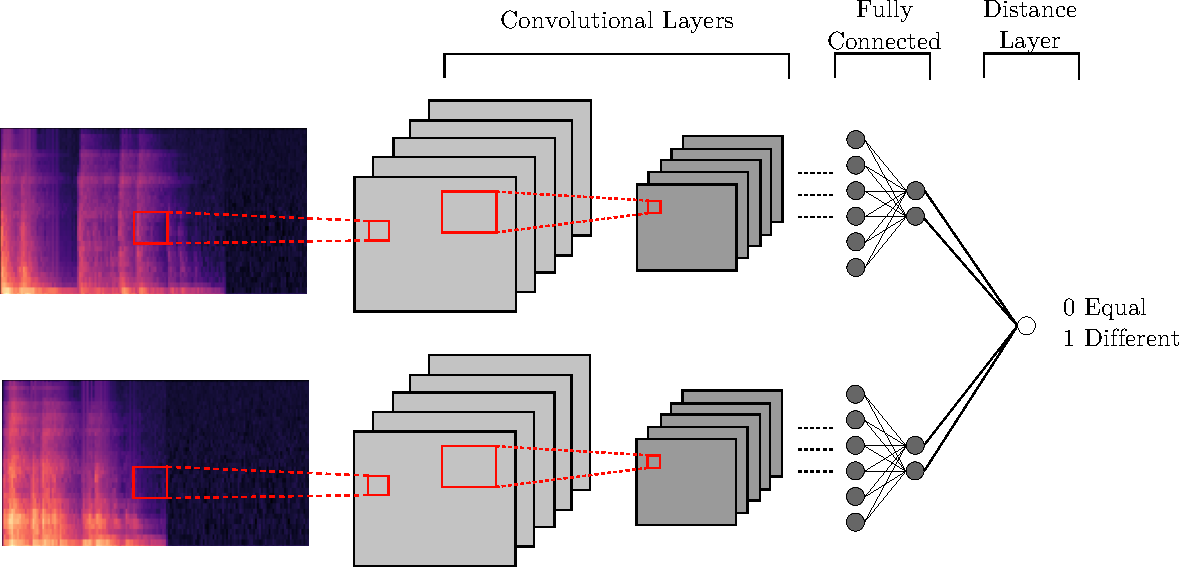
\includegraphics[width=\linewidth]{img/prai/Siamese_approach}
	\caption{Proposed approach.}
	\label{proposed_approach}
	% i mel spect sono rndy_d4st_chair_2.wav e chair_d6h0_side_5.wav
	
\end{figure*}
\subsection{Feature Extraction}
The example provided to the system are preprocessed in a features extraction stage that computes the log mel-energies. These features have been chosen as they are very popular for computational audio analysis \cite{gemmeke2013exemplar,parascandolo2017convolutional,mesaros2010acoustic}.
In particular, for this work the log mel-energies have been computed as follows.
First the signals were padded with some AWGN samples to the length of the longest audio event present in the dataset in order to work with the designed neural network.
Then the audio has been downsampled to 16 kHz and normalized. After that signal has been segmented in frames 40 ms long overlapped
by 20 ms and multiplied with a Hamming window. Discrete Fourier Transform (DFT) is calculated and the absolute value is filtered with a filterbank composed of 40 triangular filters uniformly spaced on the mel scale. At the end each audio event is represented as a matrix $X$ of shape $40\times159$.  

\subsection{Network Architecture}
As shown in \figref{proposed_approach}, the architecture explored here for the twin networks consists of $L_c$ convolutional layers followed by a max pooling. After the convolutional part, there are $L_f$ fully connected layers. After each convolutional and fully-connected layers a \textsl{batch normalization} on features map is applied followed by a \textsl{Leaky ReLU} activation function.
See \secref{sec:Results} for details about the best performing network. 



\subsection{Dataset}
All the instances related to the fall events of the R0 room (\secref{sec:dataset}) has been used in this work. In order to achieve a data augmentation, the instances recorded with all the microphones used during the creation of the dataset has been used:
\begin{itemize}
	\item one microphone array composed of 3 microphones (here taken as single microphones);
	\item 2 prototype of Floor Acoustic Sensor: the first, from now on indicated with FAS, was widely described and used in previous works \cite{Principi2016a} (\figref{fig:FAS}). For the second the only difference is the microphone used inside\footnote{RODE Lavalier: http://en.rode.com/microphones/lavalier.} that is characterized by an omni-directional directivity pattern instead of hyper-cardioid pattern.
\end{itemize}

\tableref{tab:numDataset} shows the number of instances for each class used in this work considering only audio recorded with FAS. 
%\begin{figure}
%	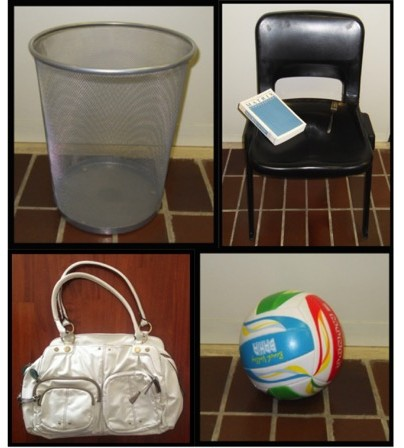
\includegraphics[width=\linewidth]{images/oggetti_cadute3.jpeg}
%	\caption{Objects used during the data acquisition camping.}
%	\label{fig:objects}
%\end{figure}
%\begin{figure}
%	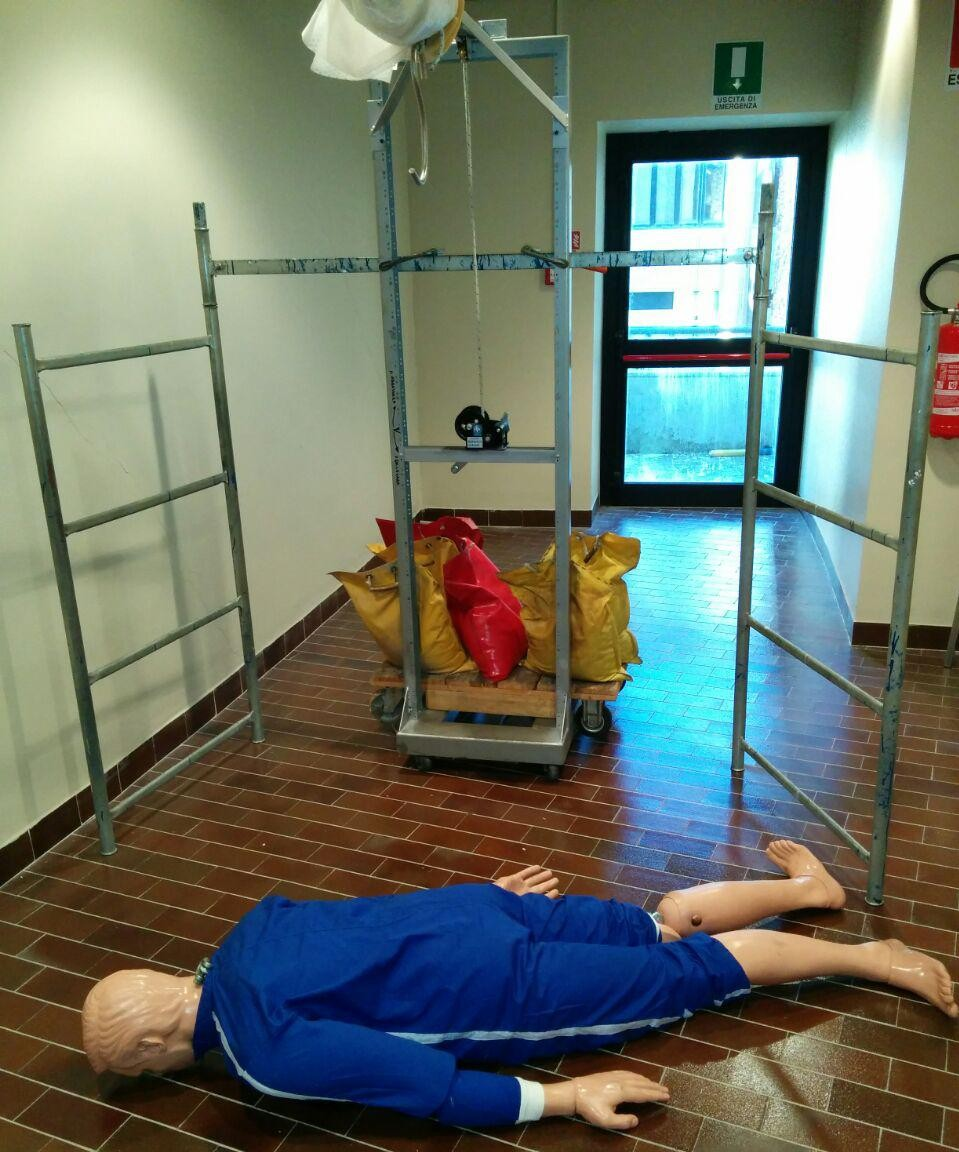
\includegraphics[width=\linewidth]{images/impalcatura.jpg}
%	\caption{Mimikin doll used to simulate the human falls.}
%	\label{fig:mimikin_doll}
%\end{figure}

\begin{table}[ht]
	\caption{Composition  of the dataset.}
	\label{tab:numDataset}
	\begin{center}
		%		\begin{tabular}[ht]{c>{\centering}m{5cm}c}
		\begin{tabular}[ht]{c|c|c}	
			\hline
			\textbf{Class} & \textbf{Nr. of occurrences} & \textbf{Total length (s)} \\ %\cline{2-5} 
			%& \hspace{8pt}Clean\hspace{8pt}  & \hspace{6pt}Clean\hspace{6pt}   \\ 
			\hline
			Basket      			& 64    &   86    	\\
			Fork        			& 64    &   82     	\\
			Ball       				& 64    &   129     \\
			Book        			& 64    &   63    	\\
			Bag         			& 64    &   57     	\\
			Chair       			& 96    &   157     \\
			$\,$ Human Falls $\,$ 	& 44    &   76     	\\
			%Human Activity  		& 665   &   1218     \\
			%Music					& 776   &	1498	\\
			%				 Classic Music       	& 441   &   882     \\
			%				 Rock Music       		& 335   &   616     \\
			\hline
		\end{tabular}
	\end{center}
\end{table}


\section{Experiments}
\label{sec:experiments}


Two methods previously described have been taken as a baseline for the comparison:
in \secref{sec:biclass_svm} a supervised approach based on bi-class SVM able to discriminate fall event from  non-fall event was employed. In this works the training set was composed of labeled data representing fall and non-fall event. In \secref{sec:ocsvm_approach} instead, an unsupervised method based on OCSVM was presented. In this case the training set was composed only from background that comprises human daily activities sounds, classical and rock music played from a loudspeaker.
.
For a correct comparison baseline, experiments have been repeated using the same data employed here for the SNN %but with some difference dependent on the type of the algorithm 
as described below \secref{sec:dataselection}.

\subsubsection{Data Selection}
\label{sec:dataselection}
All the experiments have been conducted with three-way data split and a 10 folds cross-validation strategy. In particular, for each fold, the data has been divided in 90\% for indicated, 5\% for validation and 5\% for the test, so in each set, all the classes indicated in the \tableref{tab:numDataset}, are present in a balanced way. Since here we approach the problem as a binary classification, this has led, of course, to an imbalance between the human fall and the rest% detto perchè poi mi serve per giustiicare i fatto dela confusion matrix cumulativa 
.
Because each evaluated approach differs from the other, it was necessary to select the data for each of them. To keep the various experiments comparable to each other, starting from the set above, we have constructed the various data sets for each approach as follows:
\begin{itemize}
	\item SNN: first all the signals corresponding to the human fall class have been removed from the training set. Inasmuch as the Siamese network works with paired inputs we generated all the combinations, without repetitions, between all the training examples and then randomly 80000 pairs were selected. In prediction phase, the Siamese Network needs a template to classify the events, so the development set has been subdivided in sub-test: in each of these a human fall present in the validation set has been paired with all the other events present in the same set. In the test, instead, a single human fall was selected randomly to be used as a template for each fold. This was done to keep the test set comparable between the different methods;
	\item SVM: no changes have been made to the lists;
	\item SVM-unbalanced: in the training set only a human fall has been left;
	\item OCSVM: as this is an unsupervised method all the signals corresponding to the human fall class have been removed from the training set.
\end{itemize}
For each method, the development and test set have been used only the FAS signals while the training set has been augmented with the instances of the events recorded with all others the microphones. 



\subsubsection{Validation and Evaluation}

The performances of the compared algorithm have been evaluated in term of $ F_1 -Measure$ referred to the human fall class. Due to the unbalanced nature of development and test set, the metric has been computed starting from a normalized confusion matrix. In particular, for the final evaluation, all the absolute confusion matrices coming from each fold have been summed. The cumulative confusion matrix has been then normalized and the final  $ F_1 -Measure$ was computed from it. 

To optimize the hyper-parameters of the methods the following strategies have been adopted:
\begin{itemize}
	\item for the SNN a small random search of 30 network configurations has been performed. The hyper-parameters varied during the search are reported in \tableref{tab:random_search_params}.
	The search of the threshold value of the output layer of the network which yielded the best $ F_1 -Measure$ has been performed on the validation set.
	%	 During the computation of the $ F_1 -Measure$ on the development set, optimum threshold search for the output layer of the network have been performed.
	The threshold found in this way was then used for the test of the same fold;
	\item for the SVM methods a grid search strategy has been adopted to optimize the parameters. In particular the parameters have assumed values in the ranges  $\{ 2^{-5},2^{-3},\ldots,2^{15} \}$ for $ C $ (SVM) and $ \nu $ (OCSVM), $\{ 2^{-15},\\2^{-13},\ldots,2^{3} \}$ for $ \gamma $ (both SVM and OCSVM) and  $\{ 1,2,\\\ldots,64 \}$ for the number of mixture of the GMM-UBM. 
	The parameter's values that led to the highest result were then used during the test of the same fold.
\end{itemize}

For the Siamese network, a Glorot uniform weight initializer has been used for all layers. Adadelta has been used as optimizer algorithm with default initial parameters \cite{zeiler2012adadelta}. Different values of learning rate decay have been tried in the random-search.
We trained the network for a maximum of 300 epochs, but an early stopping on the $ F_1 -Measure$ has been used to interrupt training if there were no improvements for 25 consecutive epochs. At the ends, the model corresponding to the epoch that gave the best result was selected for the evaluation on the test set.

\begin{table}[ht]
	\caption{Hyper-parameters optimized in the random-search phase, and their range.}\label{tab:random_search_params}
	\centering
	
	\begin{tabular} {|K{4cm}|K{4cm}|}
		\hline
		\textbf{Parameter} 		& \textbf{Range} \\  
		\hline
		Cnn layer Nr. 	& [2-5]		                          \\
		\hline
		Kernel shape 	& [3x3-9x9]  \footnotemark[3]      \\
		\hline									
		Kernel Nr. 		& [8-256]	                            \\
		\hline                      
		MLP layers Nr. 	&	[1-5]	                          \\
		\hline
		MLP layers dim.	&[30-8000]                            \\
		\hline
		Stride & [1x1-2x2]			                          \\
		\hline
		Dilation & [1x1-20x20]\footnotemark[3]   \\
		\hline
		Batch size	&	[100-2000]                                    						\\
		\hline 
		Max pool shape & [1x1-5x5]\footnotemark[3]      \\
		\hline
		Dropout & [Yes-No]     \tablefootnote{For all layers.}               \\
		\hline
		Drop rate	&	[0.3-0.8]                         \\
		\hline
		Learning rate decay	&	[$0$-$0.2$] \% \tablefootnote{After each epoch.}    \\
		\hline                
		Batch normalization	&	[Yes-No]                    \\
		\hline
		
	\end{tabular}
\end{table}

\footnotetext[5]{Also not squared shape has been used.}

\footnotetext[6]{Value in the square brackets represents the value adopted for each layer.}

\section{Results}
\label{sec:Results}
The results obtained for each method are reported in \figref{fig:results_f1}. The figure shows the $ F_1 -Measure$, false negative rate (miss rate) and false positive rate (false alarm rate) referred to the human fall class. It is clear that the supervised SVM method outperforms all other in terms of  $ F_1 -Measure$ as expected. The OCSVM instead is the worst method if used in this context, because its training procedure does not include any human fall, but the normality model is composed of others types of falls, making it difficult to identify the human fall as ``novelty''. The Siamese and the SVM-unbalanced, which start from the same data for the training, are classified in the intermediate positions as expected. However, we note that the proposed approach achieves a better result, exceeding the $ F_1 -Measure$ of SVM-unbalanced of about 11\%. 

As the fall detection is a task that needs to give a higher weight to the miss with respect to the false alarm, \figref{fig:results_fn_fp} reports those metrics. 
Here can be seen that both SVMs methods outperform the others, obtaining an optimum false alarm rate of 0\%. For the Miss rate, instead, while SVM reach a good result of 11\%, SVM-unbalanced give an unacceptable result of about 50\%.
The Siamese network behaves in an opposite manner with respect to the SVM-unbalanced. Although it has an high false alarm rate, it manages to reduce to zero the miss rate.
For a complete overview of the scores, in \cref{tab:cm_svm,tab:cm_svmo,tab:cm_ocsvm,tab:cm_ocsvm} are reported the normalized confusion matrix.

Another consideration is about the generalization capacity of these 4 methods. \figref{fig:score_val_test} reports the score achieved by the algorithms for both validation and test set in the 10 folds. 
The trends show that while for the SVM there is always a set of hyper-parameter able to achieve a 100 $ F_1 -Measure$ in validation phase, this does not happen for the SVM-unbalanced due to the lack of human falls during the training phase. Moreover, the results of validation are not always similar to the test value. The OCSVM instead, have a stable performance in validation, but they drop during the test, showing the poor generalization capacity of the algorithm. 
For the proposed method, instead, the trends in test follow closely the validation ones. This is highlighted in \figref{fig:diff_test_validation} where the trends of the differences in the results between the tests and validations score are shown.

	\begin{figure}
	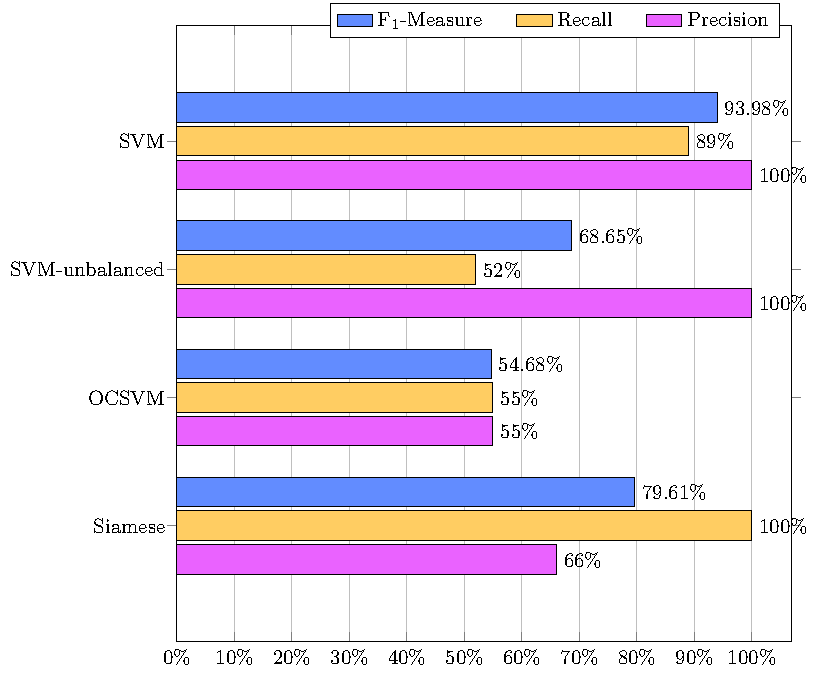
\includegraphics[width=\linewidth]{img/prai/results_f1/results_f1}
	\caption{$ F_1 -Measure$, precision and recall: the metrics are referred to the human fall class}
	\label{fig:results_f1}
\end{figure}
\begin{figure}
	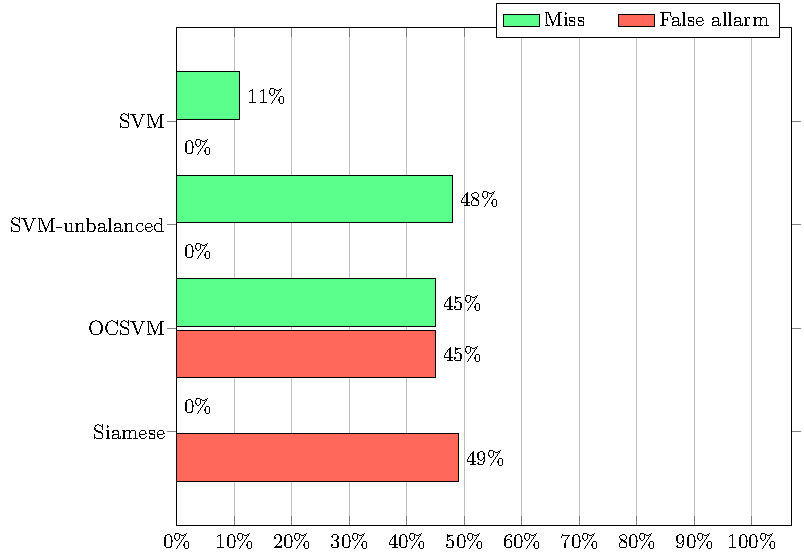
\includegraphics[width=\linewidth]{img/prai/results_fn_fp/results_fn_fp}
	\caption{Miss and false alarm rate: the metrics are referred to the human fall class}
	\label{fig:results_fn_fp}
\end{figure}
\begin{table}[ht]
	\caption{Normalized confusion matrix of the SVM approach.}
	\label{tab:cm_svm}
	\begin{center}
		
		\begin{tabular}[ht]{c|c|c}	
			\hline
			\textbf{\%} & \textbf{$\,$ Human Falls $\,$ } & \textbf{Objects} \\ %\cline{2-5} 
			
			\hline
			\textbf{$\,$ Human Falls $\,$ }     			& 89    &   11     \\
			\textbf{Objects} 								& 0    &   100     	\\
			\hline
		\end{tabular}
	\end{center}
\end{table}
\begin{table}[ht]
	\caption{Normalized confusion matrix of the SVM-unbalanced approach.}
	\label{tab:cm_svmo}
	\begin{center}
		
		\begin{tabular}[ht]{c|c|c}	
			\hline
			\textbf{\%} & \textbf{$\,$ Human Falls $\,$ } & \textbf{Objects} \\ %\cline{2-5} 
			
			\hline
			\textbf{$\,$ Human Falls $\,$ }     			& 52    &   48     \\
			\textbf{Objects} 								& 0    &   100     	\\
			\hline
		\end{tabular}
	\end{center}
\end{table}
\begin{table}[ht]
	\caption{Normalized confusion matrix of the OCSVM approach.}
	\label{tab:cm_ocsvm}
	\begin{center}
		
		\begin{tabular}[ht]{c|c|c}	
			\hline
			\textbf{\%} & \textbf{$\,$ Human Falls $\,$ } & \textbf{Objects} \\ %\cline{2-5} 
			
			\hline
			\textbf{$\,$ Human Falls $\,$ }     			& 55    &   45     \\
			\textbf{Objects} 								& 45    &   55     \\
			\hline
		\end{tabular}
	\end{center}
\end{table}
\begin{table}[ht]
	\caption{Normalized confusion matrix of the Siamese Neural Network approach.}
	\label{tab:cm_siamese}
	\begin{center}
		\begin{tabular}[ht]{c|c|c}	
			\hline
			\textbf{\%} & \textbf{$\,$ Human Falls $\,$ } & \textbf{Objects} \\ %\cline{2-5} 
			\hline
			\textbf{$\,$ Human Falls $\,$ }     			& 100    &   0     \\
			\textbf{Objects} 								& 51     &   49    \\
			\hline
		\end{tabular}
	\end{center}
\end{table}

\begin{figure}[ht]
	\centering
	\begin{subfigure}[b]{0.48\textwidth}
		\centering
		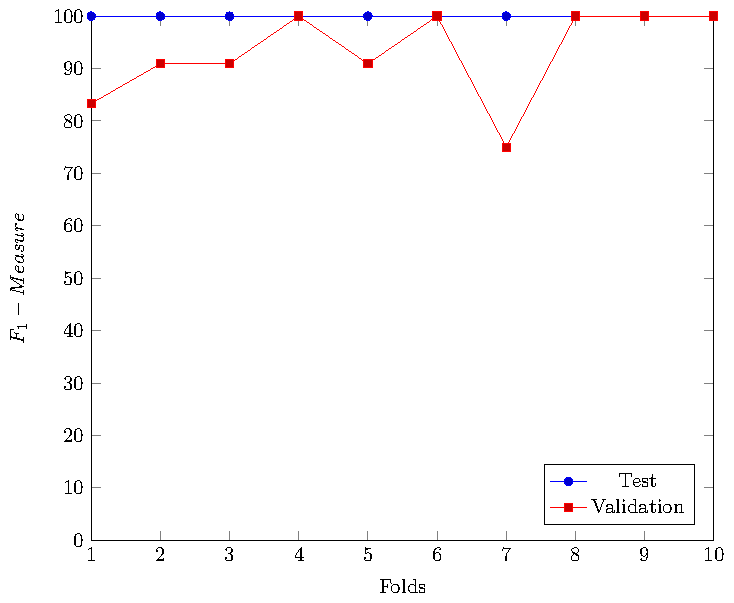
\includegraphics[width=\textwidth]{img/prai/svm_test_validation/svm_test_validation}
		\caption[Network2]%
		{{\small SVM}}    
		\label{fig:svm_val_test}
	\end{subfigure}
	\hfill
	\begin{subfigure}[b]{0.48\textwidth}  
		\centering 
		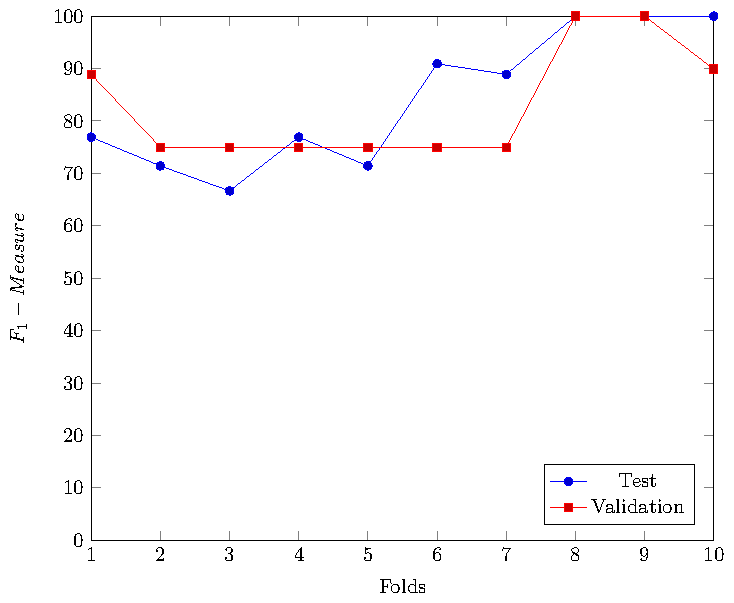
\includegraphics[width=\textwidth]{img/prai/svm_unbalanced_test_validation/svm_unbalanced_test_validation}
		\caption[]%
		{{\small SVM-unbalanced}}    
		\label{fig:svm_unb_val_test}
	\end{subfigure}
	\vskip\baselineskip
	\begin{subfigure}[b]{0.48\textwidth}   
		\centering 
		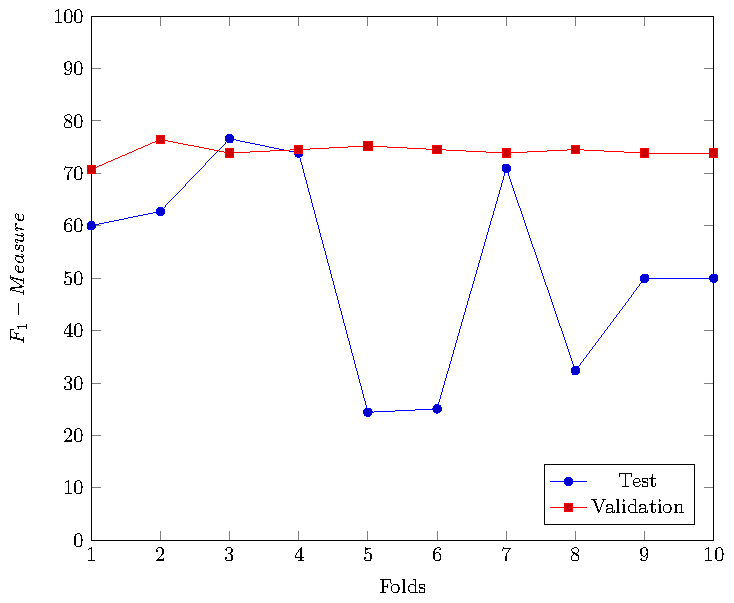
\includegraphics[width=\textwidth]{img/prai/ocsvm_test_validation/ocsvm_test_validation}
		\caption[]%
		{{\small OCSVM}}    
		\label{fig:ocsvm_val_test}
	\end{subfigure}
	\quad
	\begin{subfigure}[b]{0.48\textwidth}   
		\centering 
		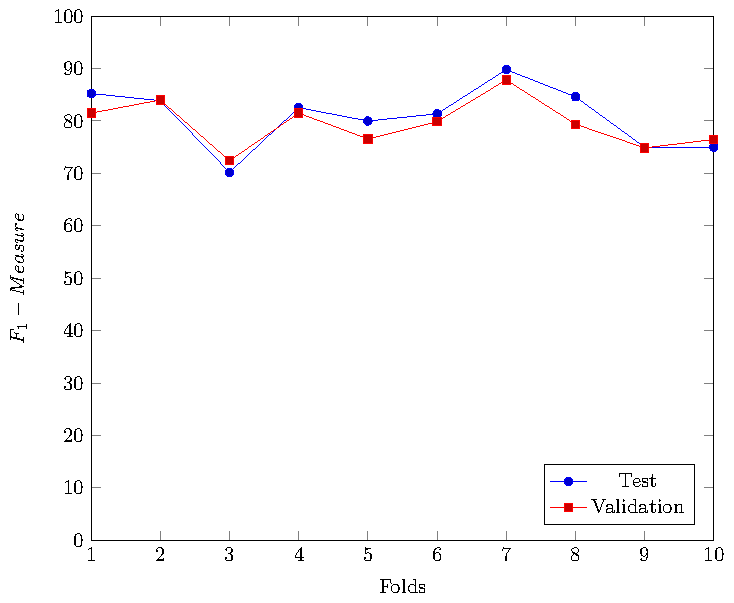
\includegraphics[width=\textwidth]{img/prai/siamese_test_validation/siamese_test_validation}
		\caption[]%
		{{\small Siamese Network}}    
		\label{fig:siamese_val_test}
	\end{subfigure}
	\caption[  ]
	{$ F_1 -Measure$ in validation and test achieved by the 4 methods in each folds} 
	\label{fig:score_val_test}
\end{figure}
\begin{figure}
	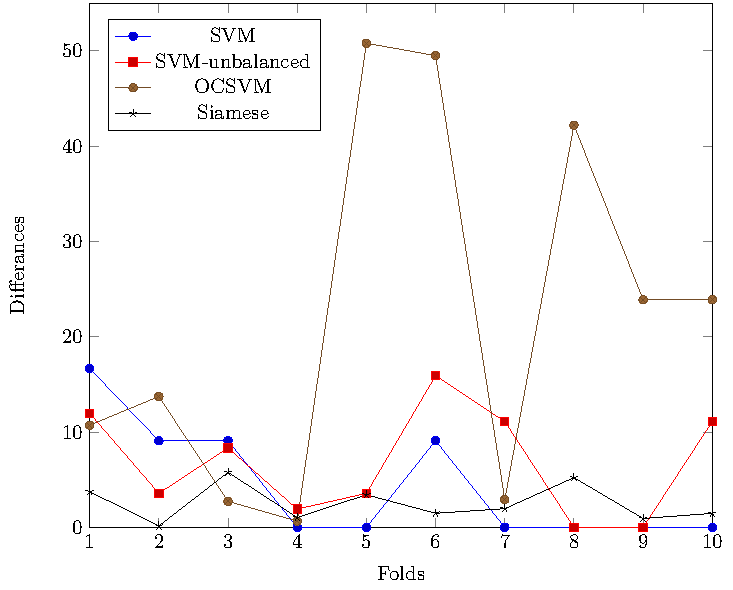
\includegraphics[width=\linewidth]{img/prai/diff_test_validation/diff_test_validation}
	\caption{Absolute value of differences between the validation and test $ F_1 -Measure$ for each fold}
	\label{fig:diff_test_validation}
\end{figure}
\begin{table}[ht]
	%	\caption{Best hyper-parameters find in random-search phase for Siamese network\tablefootnote{Value in the square brackets represents the value adopted for each layer.}.}\label{tab:opt_hyperparam}
	\caption{Best hyper-parameters find in random-search phase for Siamese network\protect\footnotemark[6].}\label{tab:opt_hyperparam}
	\centering
	
	\begin{tabular} {c | c}
		\hline
		\textbf{Parameter} 		& \textbf{Value} \\  
		\hline
		Cnn layer Nr. 	& 4		                          \\
		\hline
		Kernel shape 	& [[3x3],[3x3],[3x3],[3x3]]     \\
		\hline									
		Kernel Nr. 		& [32,32,32,32]	                            \\
		\hline   
		Stride & [[1x1],[1x1],[1x1],[1x1]]			                          \\
		\hline
		Dilation & [[1x1],[1x1],[1x1],[1x1]]  \\
		\hline
		Max pool shape & [[2x1],[1x3],[1x2],[3x2]]     \\
		\hline                   
		MLP layers Nr. 	&	3	                          \\
		\hline
		MLP layers dim.	& [3000,300,30]                        \\
		\hline
		Batch size	&	[100]                                    						\\
		\hline 
		Dropout & [Yes]        \\
		\hline
		Drop rate	&	[0.5]                         \\
		\hline
		Learning rate decay	&	[$0.1$] \% \\
		\hline                
		Batch normalization	&	[yes,no,no,no,yes,yes,yes]                   \\
		\hline
		
	\end{tabular}
\end{table}


The Siamese Network seems to be promising. Without the needing of humans falls for training, it can reduce to zero the miss rate showing also a good generalization performance with respect to the others methods. All these elements suggest that it can be used in a real scenario, but it has to be assessed also in others conditions.
In \secref{sec:siamese_one_shot}, a method based on this work will be evaluated inserting in the test even more types of audio events and noises.
Another interesting evaluation, as future work, could be to evaluate how the system behaves if trained on different data sets with respect to the one used here, also using transfer learning techniques. This is important because it could relax the necessity of carrying out a data collection campaign in every environment in which the system is going to be installed. In addition, other types of networks such as Recurrent Neural Networks or Long Short-Term Memory that have not been explored in this work could be tested.




\section{Audio Metric Learning by using Siamese Autoencoders
for One-Shot Human Fall Detection}
\label{sec:siamese_one_shot}

As shown in \secref{sec:soa}, although the literature provides several supervised and unsupervised approaches, no solution has been proposed exploiting one-shot learning for fall detection, nor to fill the gap between simulated falls and scarcely available real human falls.